\documentclass[main.tex]{subfiles}

\begin{document}

% \textcolor{red}{Вводная лекция}

\section{Лекция 09.03.2021 (Донцов Е.В.)}

\subsection{Задача для полубесконечной трещины (продолжение), плоская трещина}

\includegraphics[width=\textwidth, page=30]{HF_slides.pdf}

\includegraphics[width=\textwidth, page=31]{HF_slides.pdf}

\includegraphics[width=\textwidth, page=32]{HF_slides.pdf}

\includegraphics[width=\textwidth, page=33]{HF_slides.pdf}

\includegraphics[width=\textwidth, page=34]{HF_slides.pdf}

\includegraphics[width=\textwidth, page=35]{HF_slides.pdf}

\includegraphics[width=\textwidth, page=36]{HF_slides.pdf}

\includegraphics[width=\textwidth, page=37]{HF_slides.pdf}

\includegraphics[width=\textwidth, page=38]{HF_slides.pdf}

\includegraphics[width=\textwidth, page=39]{HF_slides.pdf}

\includegraphics[width=\textwidth, page=40]{HF_slides.pdf}

\includegraphics[width=\textwidth, page=41]{HF_slides.pdf}

\includegraphics[width=\textwidth, page=42]{HF_slides.pdf}

\includegraphics[width=\textwidth, page=43]{HF_slides.pdf}

\includegraphics[width=\textwidth, page=44]{HF_slides.pdf}

\includegraphics[width=\textwidth, page=45]{HF_slides.pdf}

\includegraphics[width=\textwidth, page=46]{HF_slides.pdf}

\includegraphics[width=\textwidth, page=47]{HF_slides.pdf}

\includegraphics[width=\textwidth, page=48]{HF_slides.pdf}





\end{document}